% Options for packages loaded elsewhere
\PassOptionsToPackage{unicode}{hyperref}
\PassOptionsToPackage{hyphens}{url}

%
\documentclass[ignorenonframetext, ]{beamer}
% \usepackage{showframe}
% ---------------------------------------------------------------%
\usetheme[]{Copenhagen}
\useoutertheme{infolines}
\setbeamertemplate{navigation symbols}{}
\usepackage{subcaption}
\usepackage{graphicx}
\usepackage{pgfpages}
\usepackage{soul}
% Prevent slide breaks in the middle of a paragraph
\usepackage{amsmath,amssymb}
% Use upquote if available, for straight quotes in verbatim environments
\IfFileExists{upquote.sty}{\usepackage{upquote}}{}
\providecommand{\tightlist}{%
  \setlength{\itemsep}{0pt}\setlength{\parskip}{0pt}}
\setcounter{secnumdepth}{-\maxdimen} % remove section numbering
\usepackage{tikz-cd}
\usepackage{adjustbox}

% `calc` is necessary to draw curved arrows.
\usetikzlibrary{calc}
% `pathmorphing` is necessary to draw squiggly arrows.
\usetikzlibrary{decorations.pathmorphing}

% A TikZ style for curved arrows of a fixed height, due to AndréC.
\tikzset{curve/.style={settings={#1},to path={(\tikztostart)
    .. controls ($(\tikztostart)!\pv{pos}!(\tikztotarget)!\pv{height}!270:(\tikztotarget)$)
    and ($(\tikztostart)!1-\pv{pos}!(\tikztotarget)!\pv{height}!270:(\tikztotarget)$)
    .. (\tikztotarget)\tikztonodes}},
    settings/.code={\tikzset{quiver/.cd,#1}
        \def\pv##1{\pgfkeysvalueof{/tikz/quiver/##1}}},
    quiver/.cd,pos/.initial=0.35,height/.initial=0}

% TikZ arrowhead/tail styles.
\tikzset{tail reversed/.code={\pgfsetarrowsstart{tikzcd to}}}
\tikzset{2tail/.code={\pgfsetarrowsstart{Implies[reversed]}}}
\tikzset{2tail reversed/.code={\pgfsetarrowsstart{Implies}}}
% TikZ arrow styles.
\tikzset{no body/.style={/tikz/dash pattern=on 0 off 1mm}}


\title{Niels Bohr on the Knowing Subject}
\author{Hans Halvorson}
\date{June 18, 2024}

%% TO DO: Rovelli relationalism

%% TO DO: stokken

%% never ending struggle for proper relation between content and
%% frame 1953

\begin{document}
\frame{\titlepage}

\section{Introduction}

\begin{frame}{Why do we find Bohr obscure?}

  When contemporary physicists and analytic philosophers read Bohr,
  they are turned off by his ``jibber jabber''

  \vfill ``Volition and causation are equally indispensable elements
  in the relationship between subject and object, which is the most
  central problem of epistemology [erkendelsesproblemets kerne].''

\end{frame}

\begin{frame}{Our context versus Bohr's}

  ``A curious thing about the \ul{ontological} problem is its
  simplicity. It can be put in three Anglo-Saxon monosyllables: 'What
  is there?'\,'' \newline (Quine, ``On what there is'', p 21)

  \bigskip \bigskip ``Danish thinking has been most interested in
  \ul{psychological} and \ul{ethical} questions, and it has usually
  been critical of the practice of system-building.'' (Høffding,
  Danske Filosoffer, p 2)

 \end{frame}


 \begin{frame}{The subject-object distinction made ontological}
   
  \begin{enumerate}
  \item Heisenberg cut of the physical world into classical and
    quantum parts
  \item Wigner cut between the mental and physical
  \end{enumerate}

\end{frame}

\begin{frame}{John Bell against the shifty split}

  ``The elimination of this shifty boundary has for me always been the
  main attraction of the `pilot-wave' picture.''

  \vfill ``The first charge against `measurement', in the fundamental
  axioms of quantum mechanics, is that it anchors there the shifty
  split of the world into `system' and 'apparatus'.''
  
\end{frame}

\begin{frame}{QBism against the shifty split \newline Mermin 2012}

  \begin{figure}
    \centering 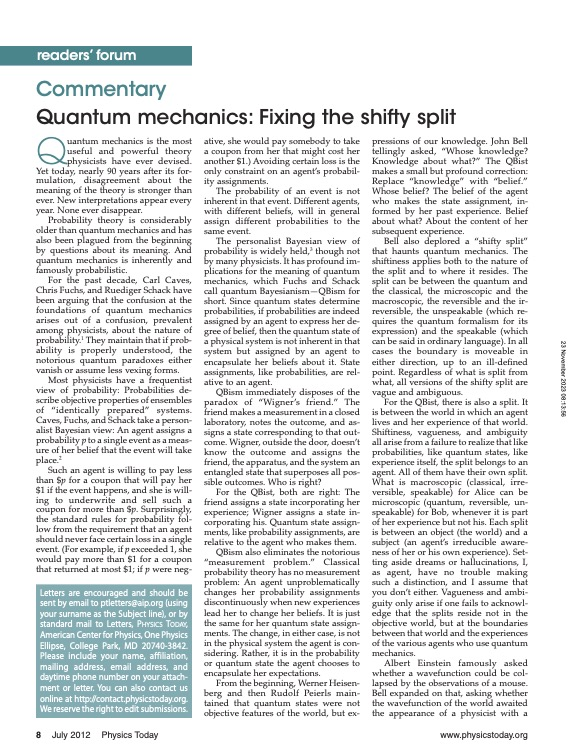
\includegraphics[scale=0.5]{mermin.jpg}
  \end{figure}  

\end{frame}

  
\begin{frame}{The split isn't an ontological thesis}

  ``For Bohr, such a cut did not originate in dynamical (ontological)
  considerations, but rather in functional (epistemological)
  considerations.'' (Camilleri and Schlosshauer 2015, p 73)

  \vfill \textbf{Thesis:} Bohr's approach to the subject-object
  distinction is rooted in 19th century epistemology and psychology
  --- especially the little-known Danish tradition
    
\end{frame}



\begin{frame}{Why didn't we see this before?}

  ``Misled by superficial coincidences, [Jammer] imagines that Bohr's
  thought has been influenced, through Høffding, by Kierkegaard and
  William James. There can be no doubt that his surmise is
  unfounded. Bohr was a completely independent thinker; from early
  youth, he developed his epistemological ideas single-handed.

  \bigskip \dots [Jammer] somehow went astray and ponderously built in
  a completely fictitious `Kierkegaard-Høffding' ideology into the
  discussion of Bohr's work.''

  \medskip (Rosenfeld, \emph{Nuclear Physics}, 1969)

\end{frame}

\begin{frame}

  \textbf{Hypothesis:} Rasmus Nielsen transformed Kierkegaard's
  epistemological and psychological ideas into something that was
  accessible to scientific thinkers such as Bohr.

  \vspace{2em}

\adjustbox{scale=0.8,center}{%
\begin{tikzcd}[ampersand replacement = \&]
  \&\&\&\& \text{H. Høffding} \\
  \text{S. Kierkegaard} \&\& \text{R. Nielsen} \&\&\&\& \text{N. Bohr} \\
  \&\&\&\& \text{Ch. Bohr} \arrow[from=2-1, to=2-3] \arrow[from=2-3,
  to=1-5] \arrow[from=2-3, to=3-5] \arrow[from=1-5, to=2-7]
  \arrow[from=3-5, to=2-7]
\end{tikzcd}
}

\end{frame}

\begin{frame}

  \begin{tikzcd}[ampersand replacement=\&]
	\&\& {\text{Poul Martin M{\o}ller}} \\
	\\
	{\text{Kierkegaard}} \&\& {\text{Rasmus Nielsen}} \\
	\\
	{\text{Christian Bohr}} \&\& {\text{H{\o}ffding}} \\
	\\
	\\
	\&\& {\text{Niels Bohr}}
        	\arrow[from=1-3, to=3-1]
	\arrow[from=3-1, to=3-3]
	\arrow[from=1-3, to=3-3]
	\arrow[from=3-1, to=5-3]
	\arrow[from=3-3, to=5-3]
	\arrow[from=3-3, to=5-1]
	\arrow[from=5-3, to=8-3]
	\arrow[from=5-1, to=8-3]
	\arrow[curve={height=-30pt}, from=1-3, to=8-3]
\end{tikzcd}




\end{frame}

\begin{frame}{Critical philosophy: The knower reflecting on itself}

  ``All theorizing must be considerate of the nature of our minds''
  \newline (Rasmus Jaksland channeling Bohr)

  \vfill ``Critical philosophy argues that a distinction must be made
  between the ways in which, according to the nature of our thought,
  we approach subjects in order to gain what for us is understanding
  --- and the nature of being itself.'' \newline (Høffding, \emph{Den
    Menneskelige Tanke}, 1910)

\end{frame}

\begin{frame}{Hegel: the subject-object distinction is \emph{aufgehoben}!}

  \begin{itemize}
  \item The Spirit can overcome the limitations of finitude that Kant
    took to constrain human subjects. (\emph{Geschichte der
      Philosophie})
  \item Through the dialectical process and an infinite reflection,
    all presuppositions can be eliminated so that Subject and Object
    become one
  \end{itemize}
  
\end{frame}


\begin{frame}{Hegel, Phenomenology of Spirit}

  ``Spirit, therefore, having won the Notion, displays its existence
  and movement in this ether of its life and is Science. It is its
  process of becoming, the circle that winds back upon itself, the
  circle that presupposes its beginning and reaches its end only in
  its beginning.''


\end{frame}

\begin{frame}{Hegel, History of Philosophy}

  ``A new epoch has arisen in the world. It would appear as if the
  World-spirit had at last succeeded in stripping off from itself all
  alien objective existence, and apprehending itself at last as
  absolute Spirit, in developing from itself what for it is objective,
  and keeping it within its own power, yet remaining at rest all the
  while. The strife of the finite self-consciousness with the absolute
  self-consciousness, which last seemed to the other to lie outside of
  itself, now comes to an end. Finite self-consciousness has ceased to
  be finite; and in this way absolute self-consciousness has, on the
  other hand, attained to the reality which it lacked before. This is
  the whole history of the world in general up to the present time,
  and the history of Philosophy in particular, the sole work of which
  is to depict this strife. Now, indeed, it seems to have reached its
  goal, when this absolute self-consciousness, which it had the work
  of representing, has ceased to be alien, and when spirit accordingly
  is realized as spirit.''

\end{frame}

\begin{frame}{Poul Martin Møller (1794--1838)}

  \begin{itemize}
  \item Hegel's philosophy introduced to Denmark by J.L. Heiberg
    (1791--1860)
  \item P.M. Møller was the first Danish philosopher to break from
    Hegel
  \item Wrote aphorisms, poetry, novellas instead of philosophy
    articles and books
  \item Teacher of Søren Kierkegaard
  \item Kierkegaard dedicated \emph{The Concept of Anxiety} to Møller
  \end{itemize}

\end{frame}  

\begin{frame}{Poul Martin Møller}

  ``What made a really deep and lasting impression on [Niels Bohr] was
  the unpretentious `Tale of a Danish Student', in which Poul Martin
  M{\o}ller has given such a delightfully humorous illustration of
  Hegelian dialectics.''

  \medskip Rosenfeld, ``Niels Bohr's contribution to epistemology'',
  1963

\end{frame}
  


\begin{frame}
  \begin{figure}
    \centering \includegraphics[scale=0.7]{eventyr.jpeg}
  \end{figure}

\end{frame}

\begin{frame}{En Dansk Students Eventyr}

  \begin{itemize}
  \item Møller's novel gives a humorous description of a young man
    (\emph{licentiaten}) who engages in an infinite reflection
  \item The target of Møller's satire: Hegel's claim that a human
    being can achieve objectivity via infinite reflection
  \item SK makes the objection explicitly.
  \item But SK doesn't leave us with any suggestions about the
    positive role of \emph{viden} or \emph{videnskab}.
  \end{itemize}

\end{frame}

\begin{frame}
\begin{figure}
  \centering 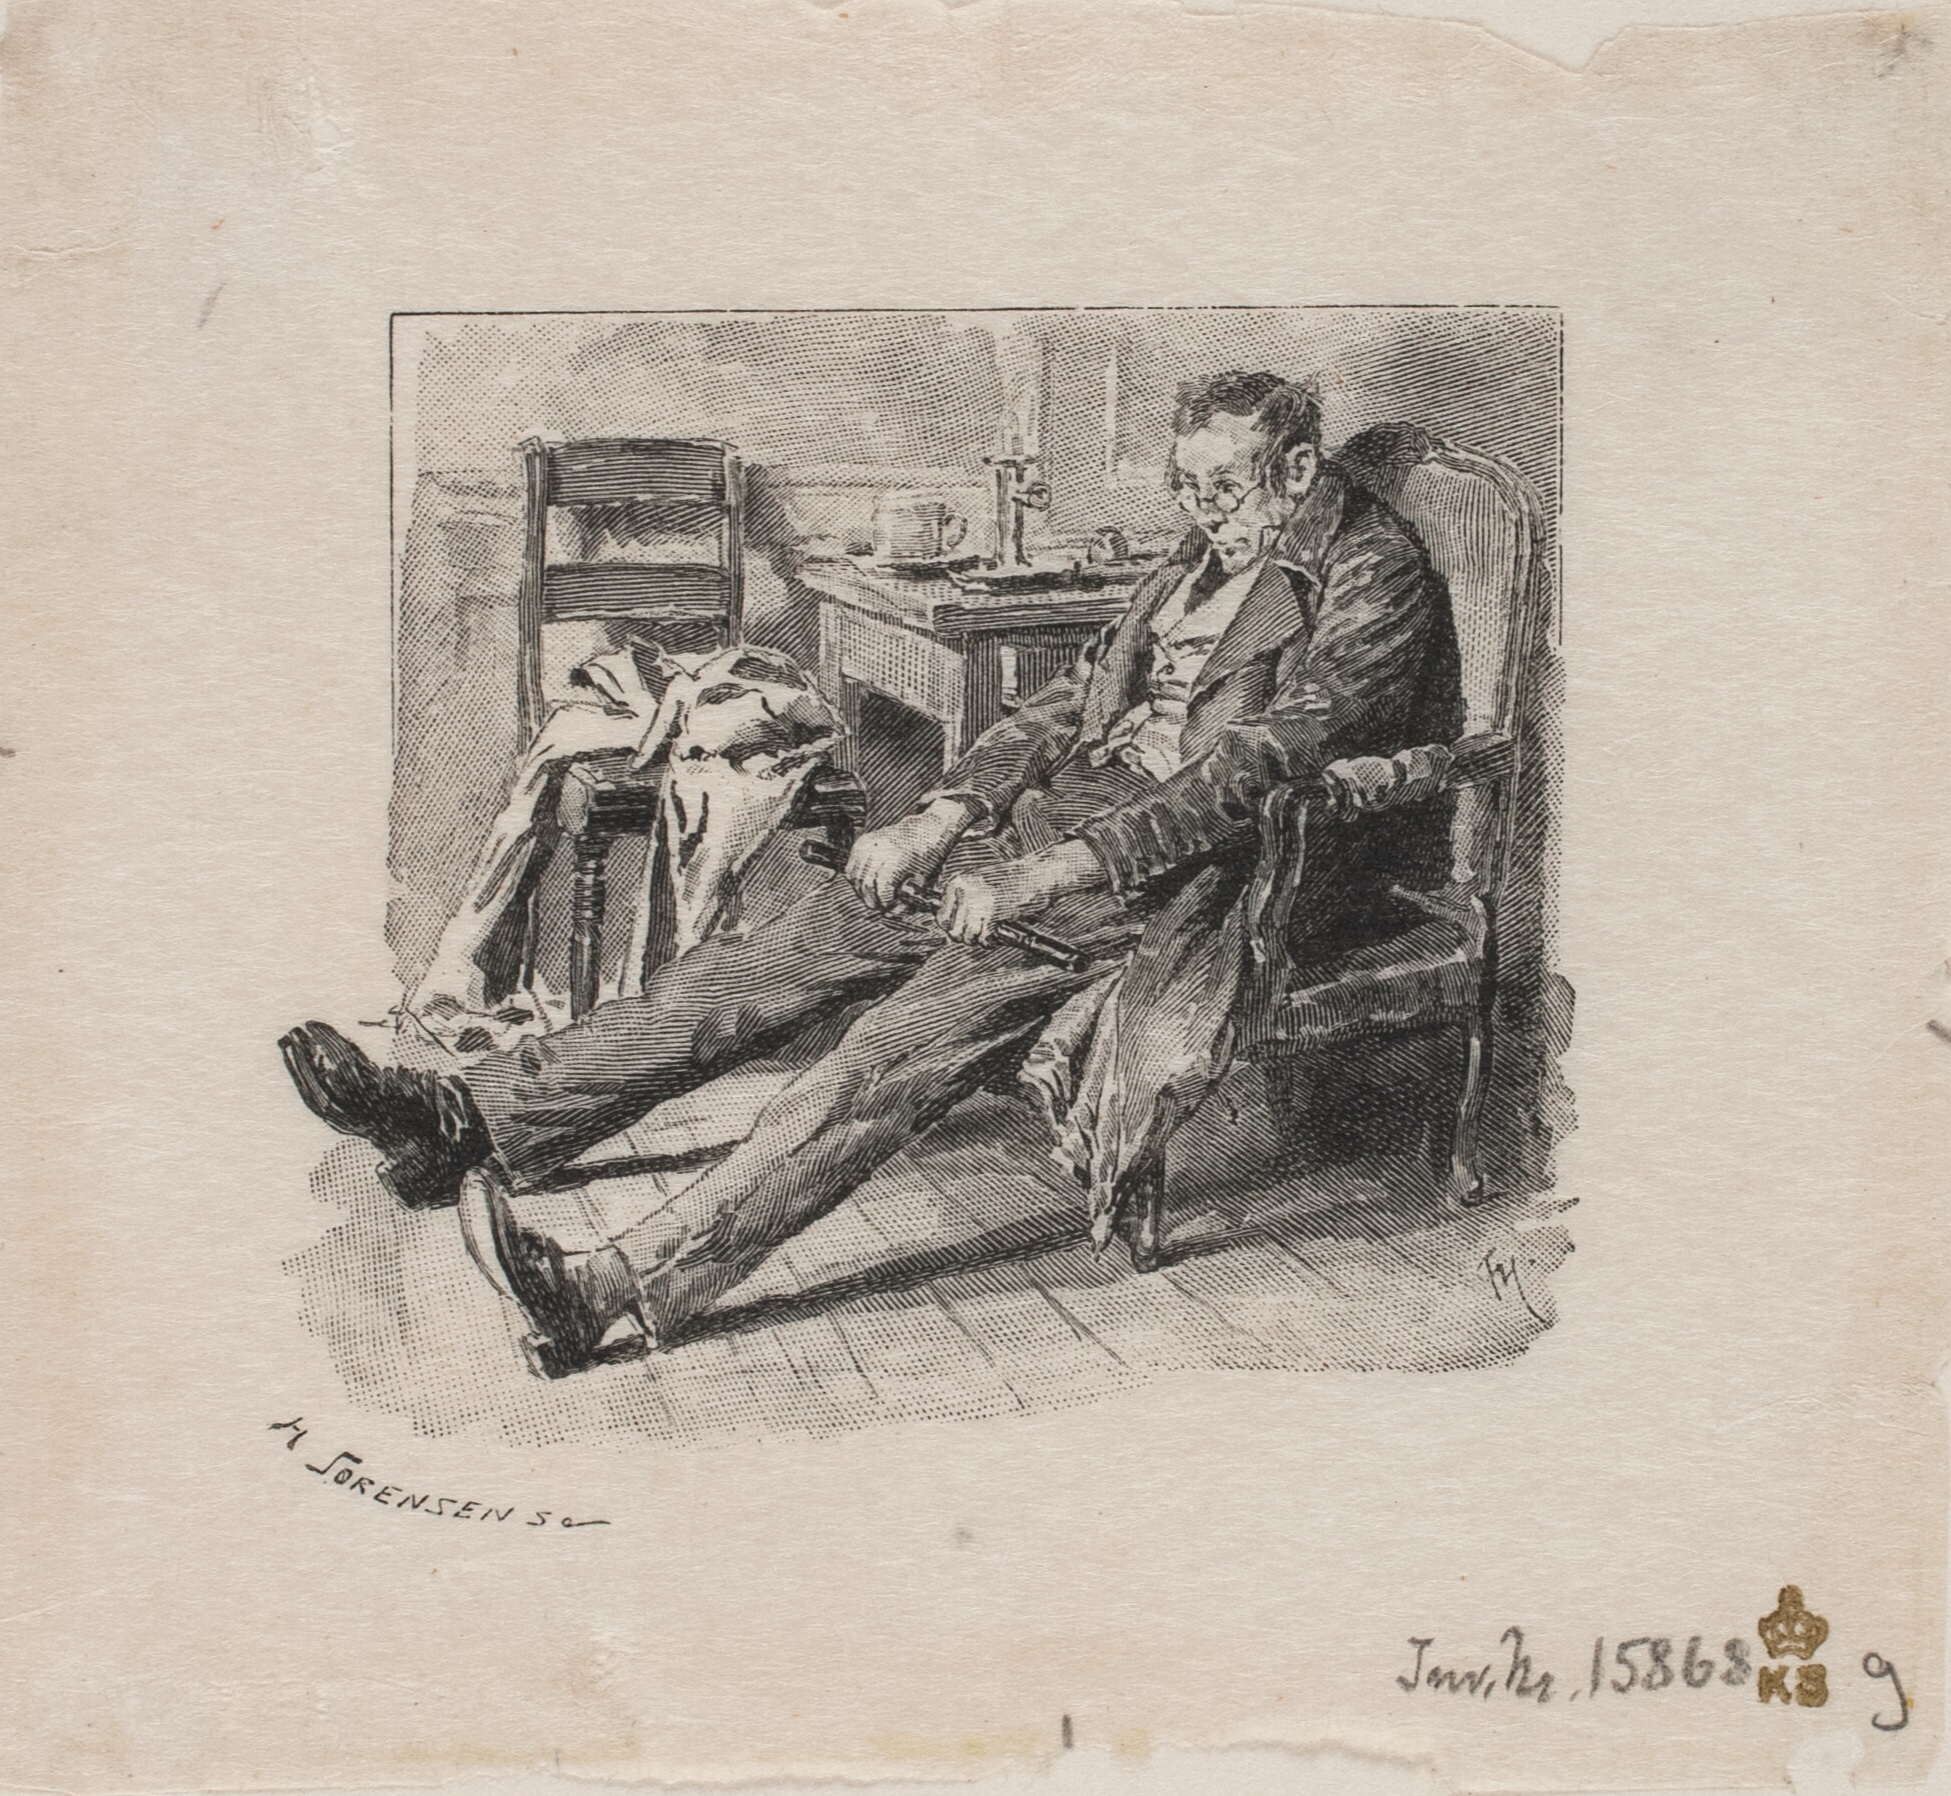
\includegraphics[scale=0.1]{licentiate.jpg}
\end{figure}
\end{frame}


\begin{frame}

  ``Father often returned, and when, in describing the the
  Licentiate's difficulties in making a decision, he found an apt
  illustration of his thoughts on the complementary features of
  psychology.''

  \medskip Hans Bohr in Rozental anthology

\end{frame}

\begin{frame}

    ``Nor do I need bring to mind the amusing story about the
    licentiate in \emph{The Adventures of a Danish Student}, which I
    related at my talk in Pasadena to elucidate the complementary use
    of terminology in psychology. The point here is, of course, that
    even though every unambiguous communication requires distinction
    between a subject and an object, the subject implied in a given
    situation can wholly or partially be included in the objective
    content of a communication about another situation.''

    \medskip NB to Delbr{\"u}ck, July 25, 1959

\end{frame}

\section{Kierkegaard}

\begin{frame}{Søren Kierkegaard (1813-1855)}

  ``It may at times occurred to you, dear reader, to doubt somewhat
  the accuracy of that familiar philosophical thesis that the outer is
  the inner and the inner is the outer.'' \newline \emph{Either-Or}

  \vfill ``Hegelian philosophy culminates in the thesis that the outer
  is the inner and the inner is the outer.'' \newline \emph{Concluding
    Unscientific Postscript}


\end{frame}



\begin{frame}

  \includegraphics[scale=0.12]{efterskrift.jpeg}


\end{frame}

\begin{frame}{The knower is a concrete individual}

  ``So we return to the two paths of reflection, and have not
  forgotten that it is an existing spirit that poses the question,
  quite simply a human being. Nor can we forget that his existing is
  just what will stop him going both ways at once, while his anxious
  question will prevent him from frivolously and fantastically
  becoming subject-object. Which of these two paths, then, is the path
  of truth for an existing spirit? For only the fantastic I-I is
  finished with both paths all at once, or proceeds methodically down
  both paths simultaneously, a gait so inhuman for an existing human
  that I do not risk recommending it.'' (Postscript, Hannay
  translation, p 162)


\end{frame}

\begin{frame}

  ``The path of objective reflection now leads to abstract thinking,
  to mathematics, to historical knowledge of various kinds, and always
  leads away from the subject, whose existence or non-existence
  becomes, and from the objective point of view quite rightly,
  infinitely indifferent --- yes, quite rightly, for as Hamlet says,
  existence and non-existence have only subjective significance. This
  path will lead maximally to a contradiction, and in so far as the
  subject fails to become wholly indifferent to himself, this only
  shows that his objective striving is not sufficiently objective.''
  (Postscript, p 163)

\end{frame}

\begin{frame}{Complementarity between reflection (overvejelse) and
    decision (afgørelse)}

  ``Once subjectivity is taken away, and passion from subjectivity,
  and infinite interest from passion, there is absolutely no decision
  [afgørelse] at all, on this problem or any other. All decision, all
  essential decision, lies in subjectivity. At no point does an
  observer (and that is what objective subjectivity is) have any
  infinite need of a decision, and at no point sees it.'' (Postscript,
  p 29)

\end{frame}

\begin{frame}{Impossibility of a final theory}

  ``There can be no system for life itself. \dots System and finality
  correspond to each other, but life is just the opposite. From an
  abstract point of view, system and existing cannot be thought
  together; because systematic thought in order to think life must
  think of it as annulled and hence not as life. Existence is the
  spacing that holds things apart; the systematic is the finality that
  joins them together.'' (Postscript, p 100)

\end{frame}

\section{Nielsen}

\begin{frame}

  \begin{itemize}
  \item Kierkegaard criticizes Hegel's epistemology, but doesn't offer
    any positive account of the role of objective knowledge
    (\emph{Viden}) in human life
  \item The forgotten link: Rasmus Nielsen developed a
    Kierkegaard-inspired philosophy of science
  \item Nielsen was originally a Hegelian, but changed completely when
    he read the \emph{Postscript}
  \end{itemize}

\end{frame}

\begin{frame}{Rasmus Nielsen (1809--1884)}

  \begin{itemize}
  \item[1857] \emph{Philosophie og Mathematik. En propædeutisk
      Afhandling}
  \item[1859] \textit{Mathematik og Dialektik}
  \item[1864] \textit{Grundideernes Logik}
  \item[1873] \textit{Natur og aand: bidrag til en med physiken
      stemmende naturphilosophie}
  \item[1880] \emph{Almindelig Videnskabslære i Grundtræk}
  \item[1881] \emph{Om det oprindelige forhold mellem religion og
      videnskab}
  \end{itemize}
    
\end{frame}

\begin{frame}{Nielsen's scientific turn}

  ``As my recent writings show, it has been my goal, for a number of
  years, to clarify and demonstrate the relationship between
  philosophy and the separate sciences as comprehensively as
  possible. The future of philosophy depends in an essential way on a
  thorough understanding and accurate determination of this
  relationship.'' (1864, p 18)
  
\end{frame}

\begin{frame}

\begin{itemize}
\item Nielsen and Sibbern alternated teaching ``det indledende
  filosofikum'' (introductory philosophy course) for many years.
  \begin{itemize}
  \item This course was mandatory for all first-year students at the
    university, in any subject.
  \end{itemize}
\item Circa 1860, students complaining that Nielsen demanded too much
  knowledge of math and science.
\end{itemize}
\end{frame}

\begin{frame}

``At first it was Rasmus Nielsen, whose enthusiastic references to
  Kierkegaard and whose rousing eloquence had the greatest influence
  on me.'' (Høffding 1909)

  \vfill

  ``No one who studies the life of the mind in nineteenth-century
  Denmark, will be able to skip over [Nielsen's] great philosophical
  writings, and everyone who got to hear his lectures at the
  university will remember him as a great awakener and a rare
  personality.'' (Brandes 1899)
  
\end{frame}

\begin{frame}

  \begin{figure}[!ht]
    \setkeys{Gin}{width=0.18\linewidth}
    \captionsetup[subfigure]{skip=0.5ex,
                             belowskip=1ex,
                             labelformat=simple}
    \renewcommand\thesubfigure{}

\subfloat[Heegaard]{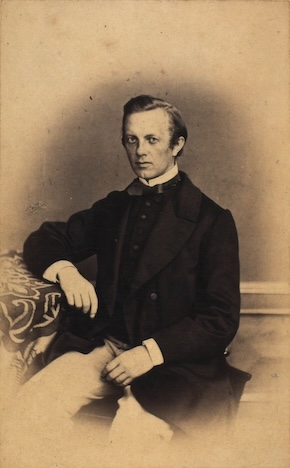
\includegraphics{heegaard.jpg}}
\hfill
\subfloat[Brandes]{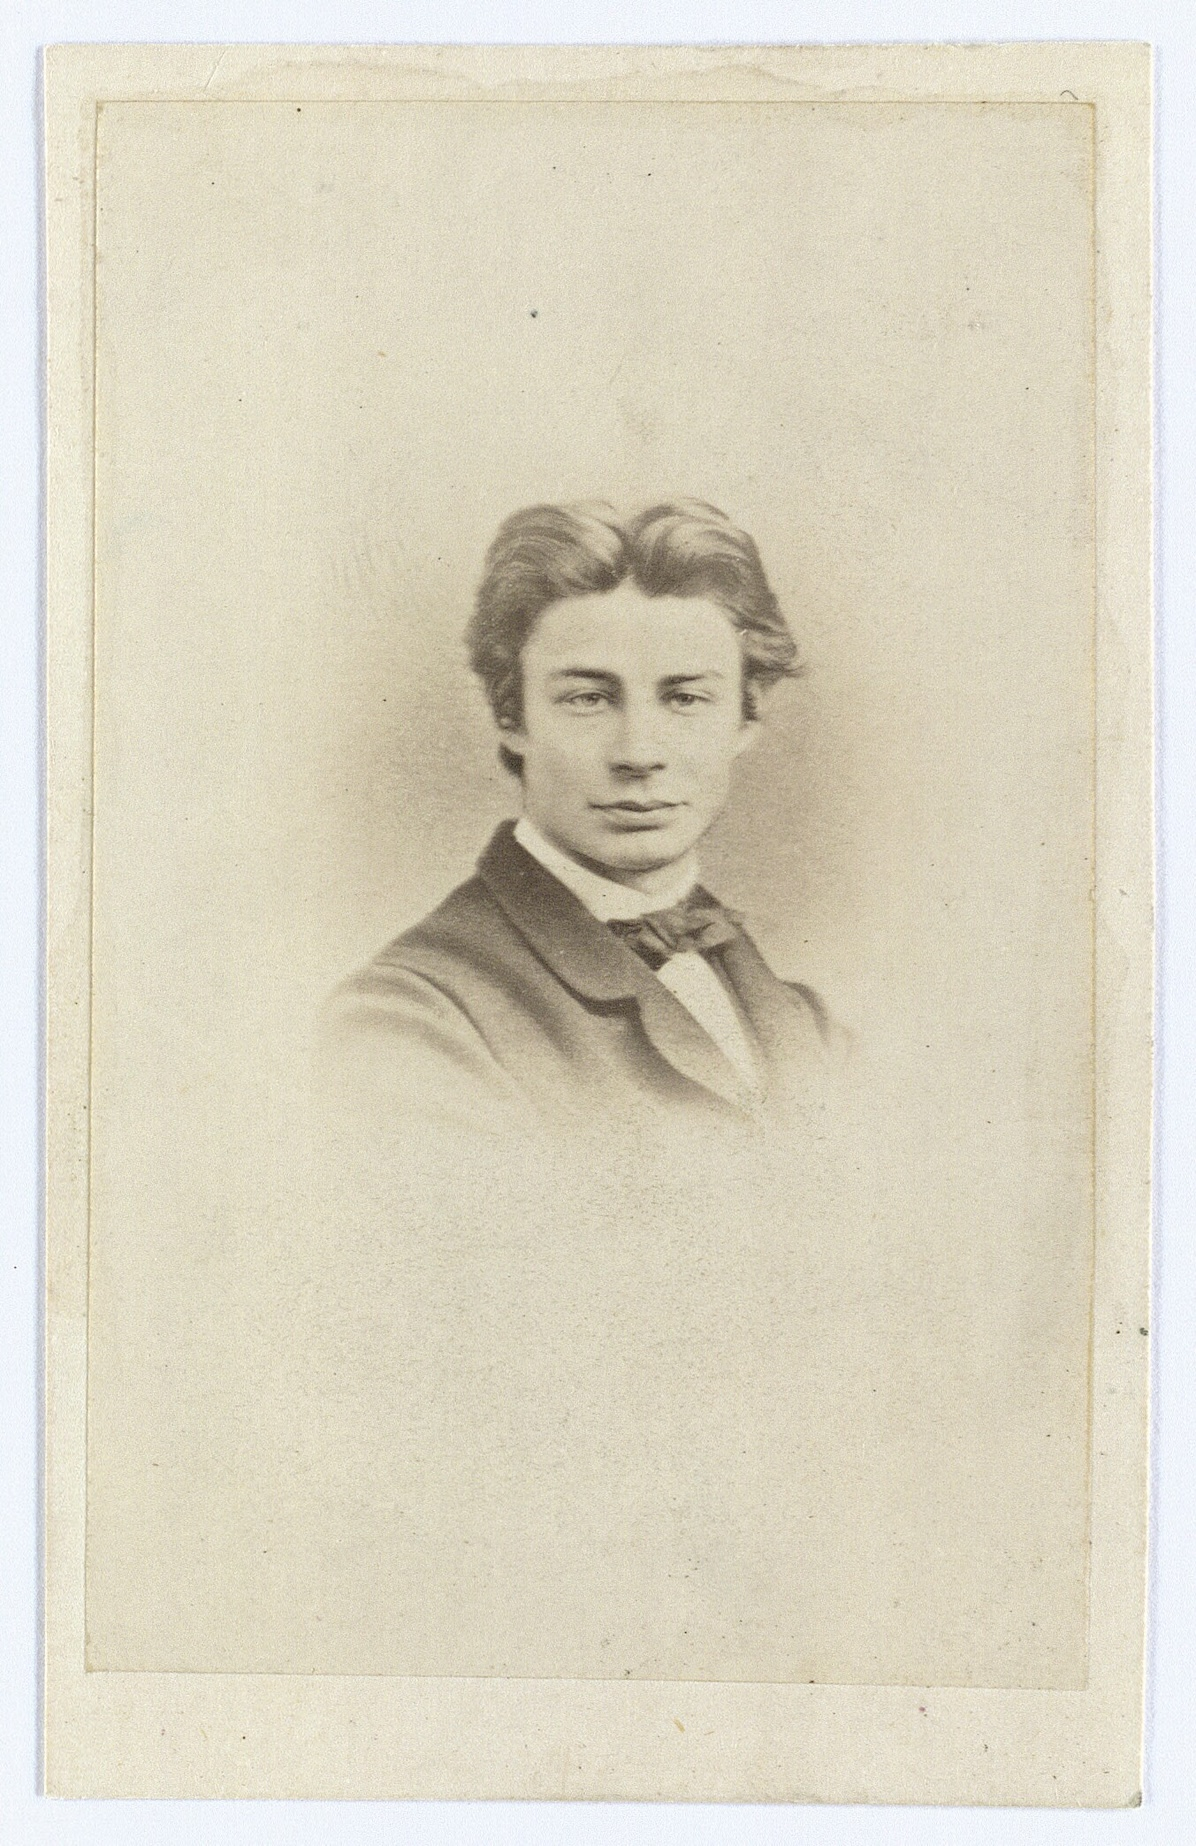
\includegraphics{brandes.jpg}}
\hfill
\subfloat[Høffding]{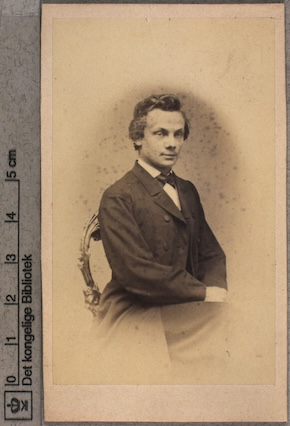
\includegraphics{høffding.jpg}}

\medskip
\subfloat[Kroman]{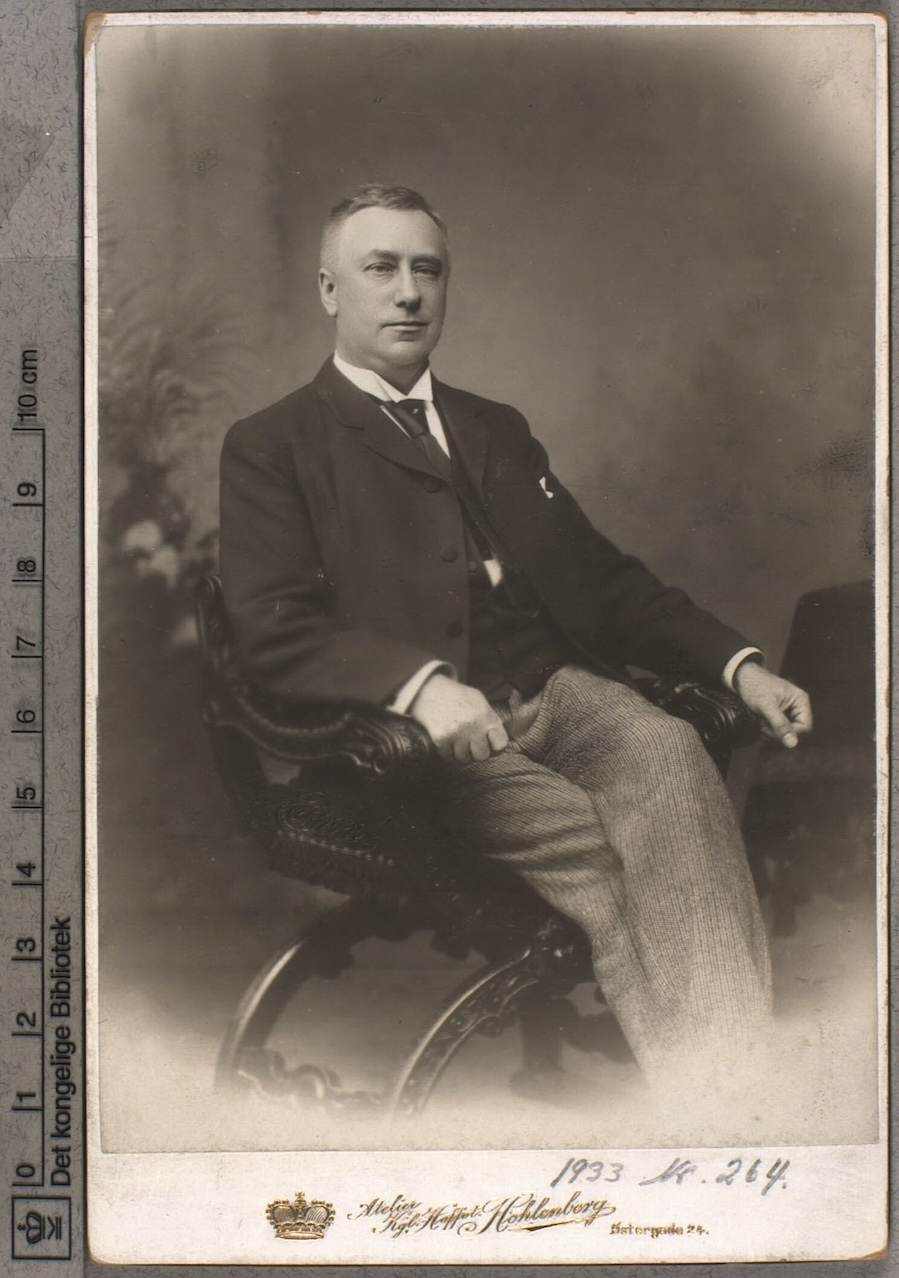
\includegraphics{kroman.jpg}}
\hfill
\subfloat[Lehman]{\includegraphics{lehman.jpg}}
\hfill
\subfloat[Ch. Bohr]{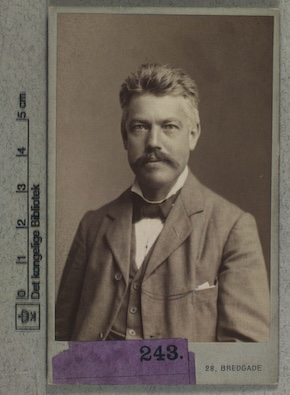
\includegraphics{christian.jpg}}
    \end{figure}

  
\end{frame}

\begin{frame}

\begin{figure}
  \centering 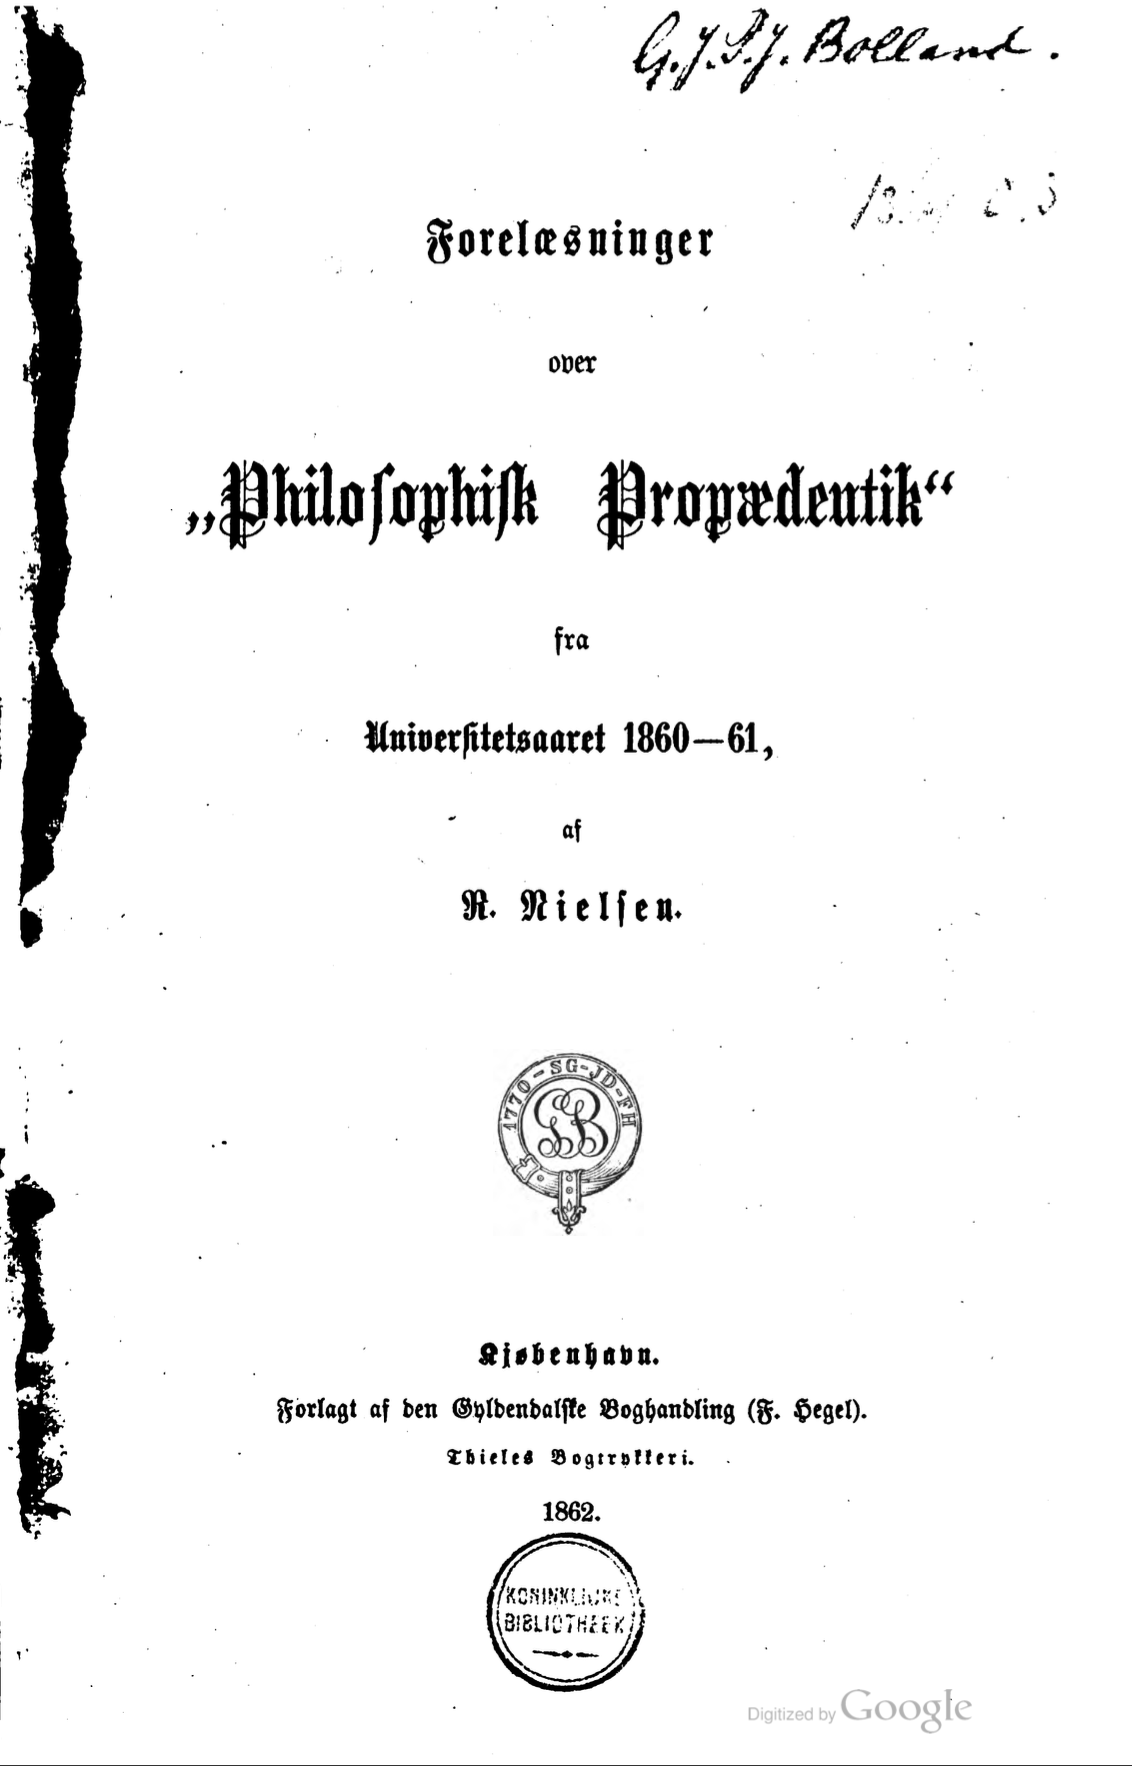
\includegraphics[scale=0.5]{prop1.png}
\end{figure}
\end{frame}

\begin{frame}

\begin{figure}
\centering
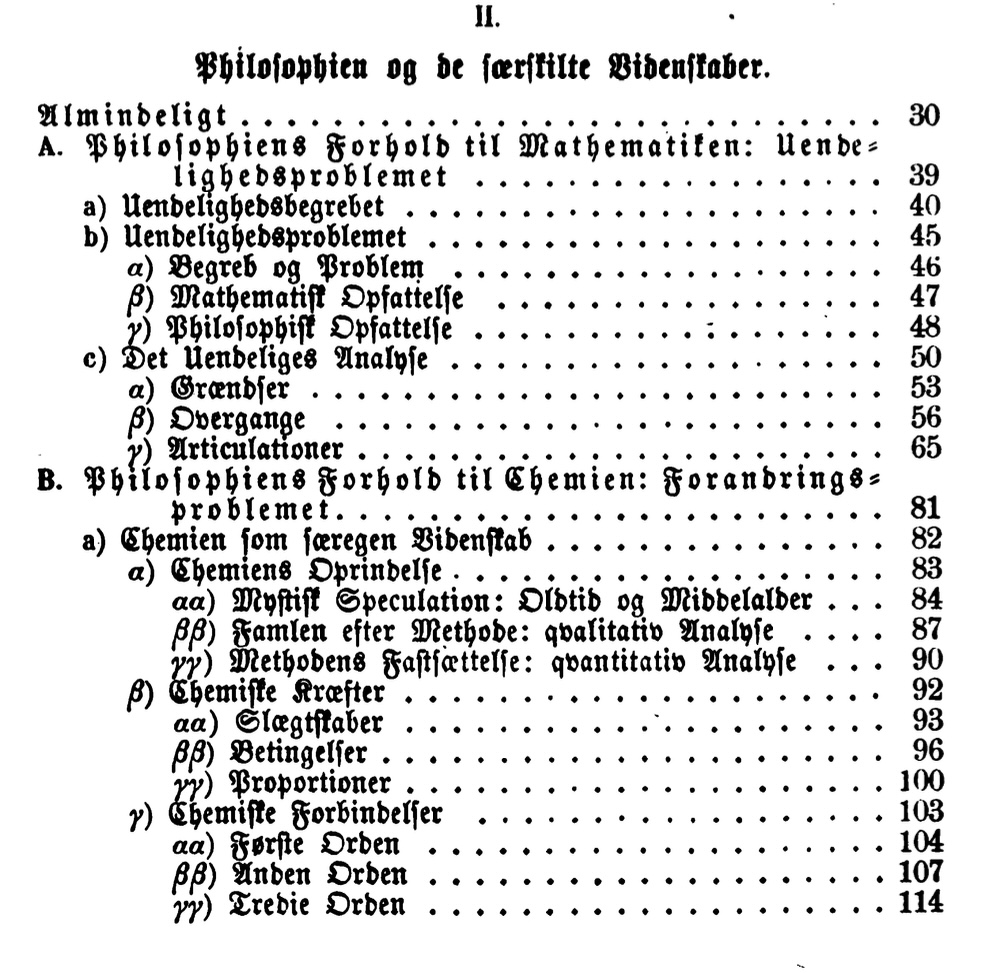
\includegraphics[scale=0.65]{prop2.jpg}
\end{figure}
\end{frame}

\begin{frame}

\begin{figure}
\centering
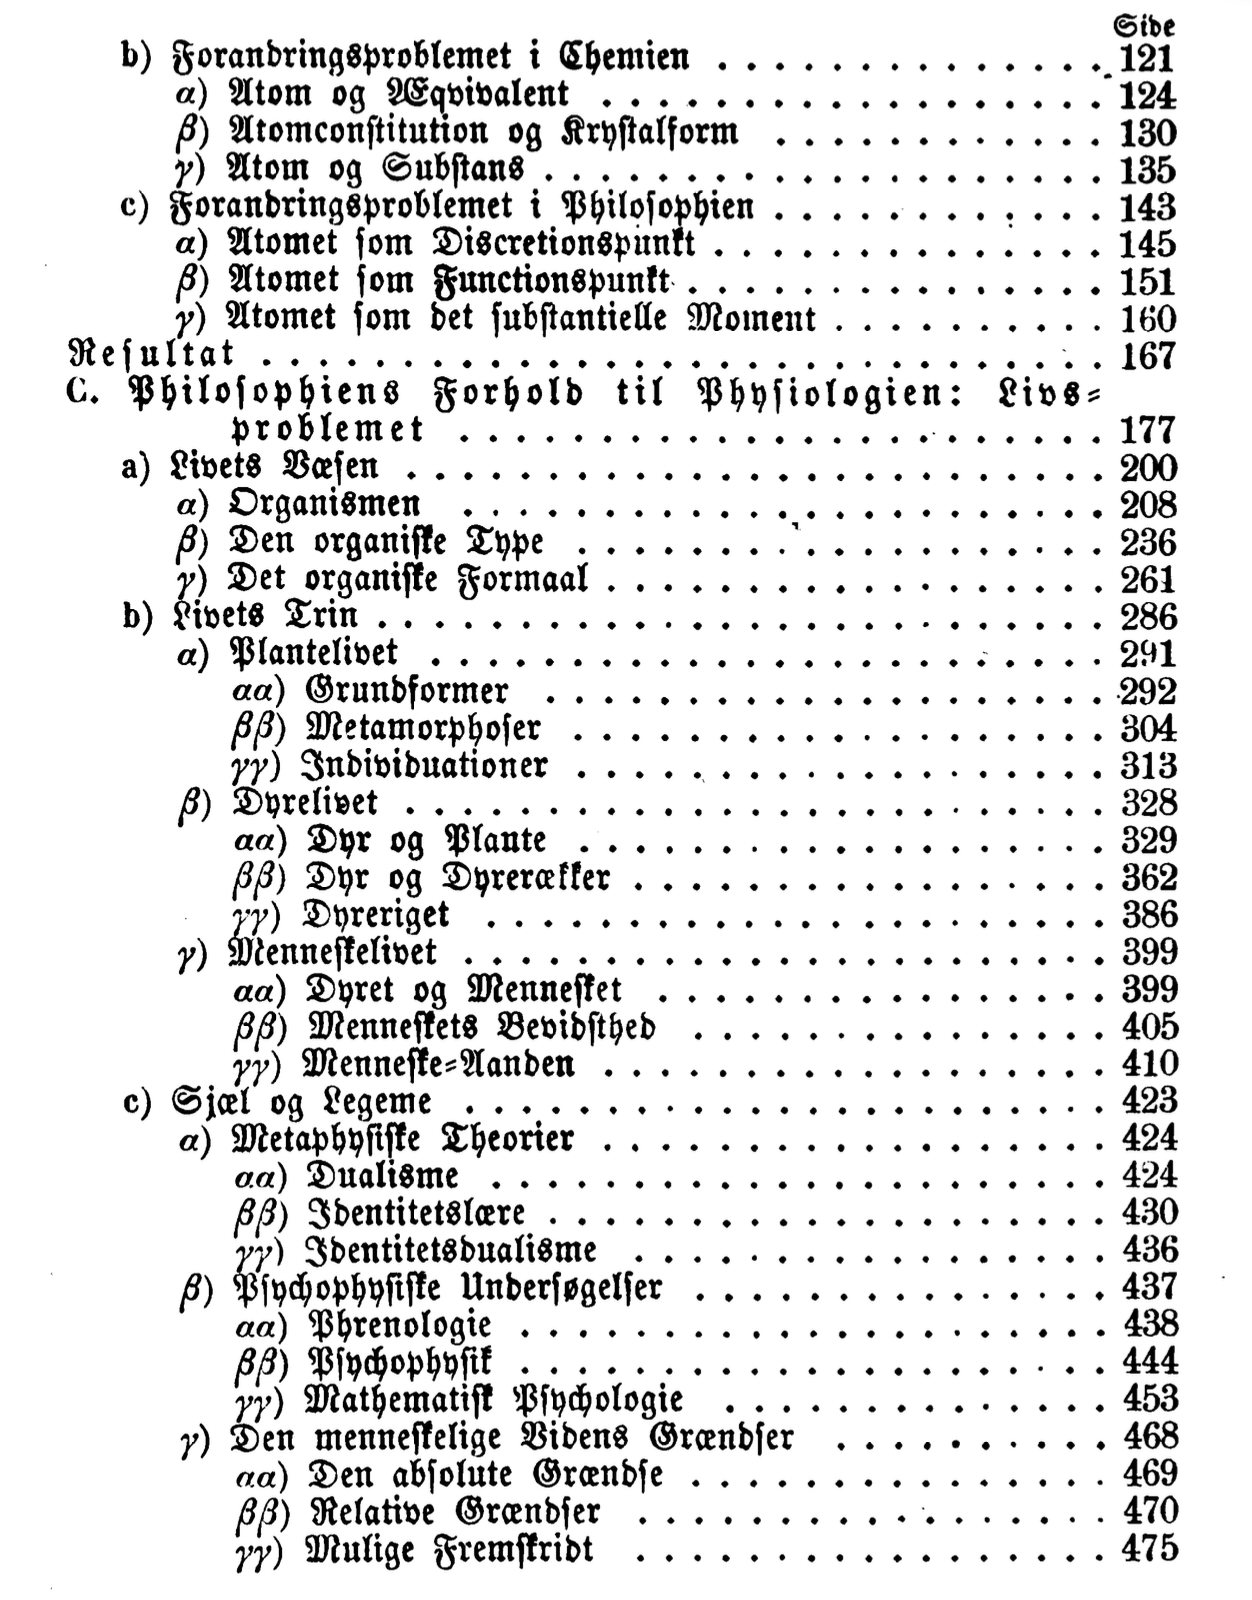
\includegraphics[scale=0.5]{prop3.jpg}

\end{figure}
\end{frame}



\begin{frame}{Objectiveringslov}

  ``No object without a corresponding objectification; it is an a
  priori law that underwrites all empiricism, a basic law that in
  science is, if possible, even more unshakable than Newton's law of
  gravity. From this it can be seen, that a critical boundary, a
  boundary line, on whose one side we have the objectivizing
  subjectivity, while the object is standing on the other side, is
  confused and meaningless.'' (1880, p 41)

\end{frame}

\begin{frame}

  The boundary between apriori and aposteriori is moveable.

  \vfill 

  ``When the boundary between apriori and empirical is supposed to be
  conceived of as definite and exact, then troubles arise.'' (1880, p
  30)


  \vfill ``A fixed, unmovable boundary line between the apriori and
  aposteriori cannot be set.'' (1880, p 37)

\end{frame}


\begin{frame}

  
  ``Admittedly it is, as far as the truths and the sense organs are
  concerned, undeniable that one and the same substratum, by being
  objectified in different systems, should appear as different
  objects; but this confirms precisely what the Basic Law says. If the
  substrate is denoted by $X$, the determinations therein by $X_o$,
  $X_1$, $X_2$, then these determinations, when expressed in the $A$
  system, would give $a_o,a_1,a_2,\dots $ and the whole corresponding
  Object would be $O_a$; in the $B$ system it would be $O_b$; in the
  $C$ system it would be $O_c$. But is this not a proof that the
  Objective cannot be recognized?  Not at all; it is precisely a proof
  of the interaction between Objective and Subjective.'' (1880, p 54)

\end{frame}


\begin{frame}

  ``Al søgen efter et sidste subjekt er i strid med målet om objektiv
  beskrivelse, som kræver en modstilling af subjekt og objekt.''
  \newline (Den menneskelige erkendelses enhed, 1960)

  \vfill ``Nielsen believed that, to describe the interrelation
  between the subjective and the objective, an infinite analysis was
  needed, since every subject presupposes an object, and every object
  in turn a subject.''  \newline (Høffding, Danske Filosoffer, p 189)

\end{frame}



\section{Høffding}

\begin{frame}{Harald Høffding}

  ``Just as form and content are abstractions, since in every act of
  cognition we have a combination of them, so it is with subject and
  object.'' (1910, p 297)

\end{frame}

\begin{frame}

  ``We could make our own subject an object for us, just as when we
  study it psychologically, e.g. to find out the forms by which it
  works in its cognition. These forms, which are systematized in the
  study of the categories of cognition, must be taken as facts. They
  are made subjects when reflection is applied to them. Every
  cognition takes place from a certain point of view, which it can be
  meaningful to ascertain [konstatere]. We then objectify the
  subject.'' (1910)


\end{frame}

\begin{frame}

  ``When we consider something as an object, we must indicate the
  nature of the subject in relation to which it exists. And when we
  consider something as a subject, we must partly seek the objective
  context that determines its nature and thereby the contents and
  forms that are at its disposal, and on the other hand we need to
  note that by this investigation we ourselves make that subject into
  an object (if it is ourselves, then for ourselves in a somewhat
  different state, at any rate at a different moment, than before). We
  never have a pure subject ($S$), but always an objectively
  determined or yet an objectified subject ($S_o$). And we never have
  a pure object ($O$), but always a subjectivized object ($O_s$). $S$
  and $O$ are mere abstractions. What we have before us is always
  $S_o$ and $O_s$.'' (1910, p 298)


\end{frame}

\begin{frame}

  ``The act of becoming self-conscious, of making one's I (one's
  conditions, one's work, one's circumstances) into an object for
  itself, can always be repeated. The I that becomes self-conscious
  can itself become the object of a new act of self-consciousness, and
  so on. Such a series $(S_1 \prec S_2 \prec S_3 \prec S_4 \dots )$
  has already been mentioned above in connection with the possibility
  of an epistemological investigation into epistemology.'' (Totalitet
  som Kategorie, p 36)

\end{frame}

\begin{frame}

  ``Den Akt at blive sig selv bevidst, gøre sit Jeg (sine Tilstande,
  sit Arbejde, sine Kaar) til Genstand for sig, kan formelt stadig
  gentages. Det Jeg, der bliver sig selv bevidst, kan selv blive
  Genstand for en ny Selvbevidsthedsakt, og saaledes fremdeles. En
  saadan Række $(S_1 \{ S_2 \{ S_3 \{ S4 ....)$ er allerede omtalt
  ovenfor i Anledning af Muligheden af en erkendelsesteoretisk
  Prøvelse af Erkendelsesteorien.'' (Totalitet som Kategorie, p 36)

\end{frame}

\section{Conclusion}


\begin{frame}{Open questions}

  How does Kantian critical philosophy (i.e.\ knowing the subject's
  capacities) get combined with empirical science in the 19th century?
  \begin{itemize}
  \item Helmholtz
  \item Mach
  \item Etc?
  \end{itemize}

\end{frame}

\begin{frame}{Conclusions}

  \begin{itemize}
  \item Bohr's talk about subject and object is jibber-jabber only if
    European philosophy (and literature) of the 19th century is
    jibber-jabber.
  \item I stand against those who deny the deep humanistic origins of
    scientifically fruitful ideas.
  \item Bohr's view about subject-object builds creatively on the
    tradition of Møller, Kierkegaard, Nielsen, and Høffding.
  \item Bohr's ``erkendelsesteoretisk belæring'' should be judged as a
    radical alternative to Quinean metaphilosophy rather than as a
    particular interpretation of QM (i.e.\ solution to John Bell's
    measurement problem) within the framework of Quinean
    metaphilosophy.
  \end{itemize}


\end{frame}

\begin{frame}{To do list}

  \begin{itemize}
  \item Learn the languages
  \item Read 
  \item Know the history --- science, philosophy, and culture in
    general
  \end{itemize}

\end{frame}  
  


\begin{frame}{The stick analogy}

  ``One need only remember here the sensation, often cited by
  psychologists, which every one has experienced when attempting to
  orient himself in a dark room by feeling with a stick. When the
  stick is held loosely, it appears to the sense of touch to be an
  object. When, however, it is held firmly, we lose the sensation that
  it is a foreign body, and the impression of touch becomes
  immediately localized at the point where the stick is touching the
  body under investigation.'' (The Quantum of Action and the
  Description of Nature, 1929, p 99)

\end{frame}

\begin{frame}

  ``But Bohr would also point to psychological experience in daily
  life in connection with the difficulty of distinguishing between
  subject and object, in order to facilitate understanding of the new
  situation in physics, where his view appeared too radical or
  mysterious even to many physicists. In this connection he chose as a
  particularly simple example the use of a stick when trying to find
  one's way in a dark room. Here the dividing line between subject and
  object is placed at its end, when the stick is grasped firmly,
  while, when it is loosely held, the stick appears as an object.''
  (Oskar Klein, p 92 in Rozental)

\end{frame}

\begin{frame}

  ``\dots in order to make clear the necessity of sharply separating
  the means of observation from the observed system, he would adduce
  the familiar example of the blind man's stick: If you hold a stick
  firmly in your hand, it can serve as a sort of prolongation of the
  latter to explore the surroundings by touch; but if you hold it
  loosely, it becomes itself an object whose presence is revealed to
  the hand by the sense of touch, and it loses thereby its function of
  instrument of observation.'' (Rosenfeld, p 124 in Rozental)

\end{frame}

\begin{frame}

  ``On one occasion while on a walk in the woods near Copenhagen Bohr
  picked up a stick and pointed out that, when one uses it as a probe
  and pokes various objects with it, one's feeling seems to be at the
  end of the stick, not in the hand that is holding it, although of
  course it is the hand that directly experiences the feeling. The
  stick seems like an extension of one's arm. \dots By such a simple
  observation which most people overlook, Bohr showed the attention
  that he gave to psychological questions.'' (Dirac, p 306 in
  Rozental)

\end{frame}

\begin{frame}

  ``Ordinary language, by its use of such words as thoughts and
  sentiments, admits typical complementary relation between conscious
  experiences implying a different placing of the section line between
  the observing subject and the object on which attention is focused.
  We are here presented with a close analogy to the relationship
  between atomic phenomena appearing under different experimental
  conditions and described by different physical concepts, according
  to the role played by the measuring instruments.'' \newline
  (Physical Science and the Study of Religions, 1953, p 389)

\end{frame}

\begin{frame}{}

  ``In fact, the varying separation line between subject and object,
  characteristic of different conscious experiences, is the clue to
  the consistent logical use of such contrasting notions as will,
  conscience and aspirations, each referring to equally important
  aspects of the human personality.'' \newline (Physical Science and
  the Study of Religions, 1953, p 390)

\end{frame}

\begin{frame}

  ``In emphasizing the necessity of paying proper attention to the
  placing of the object-subject separation in unambiguous
  communication, the modern development of science has created a new
  basis for the use of such words as knowledge and belief.'' (Unity of
  Knowledge, 1954, p 61)

\end{frame}




\begin{frame}{Sources}

  \begin{itemize}
  \item Pais, pp 439--441
  \item Rosenfeld, ``Niels Bohr's contribution to epistemology''
  \item Rosenfeld, Review of Max Jammer  
  \item Rozental. \textit{Niels Bohr: His Life and Work as Seen by His
      Friends and Colleagues}
  \item C.H. Koch. \textit{Den Danske Idealisme}
  \end{itemize}


\end{frame}

\begin{frame}{Rosenberg on Nielsen}

  \begin{quote} Her fremsætter Nielsen den 'Objektiveringslov', som
    senere blev et saa betydningsfuldt Led i hans Metafysik:
    Objekterne kan ikke objektivere sig selv, og da Objekter uden
    Objektivering er umulige, forudsætter Objektiviteten en
    objektiverende Subjektivitet. Paa den anden Side kan
    Subjektiviteten ikke undvære Objektiviteten, eftersom dens
    Selvbegriben og Selvmagt saa vilde blive uden Indhold.
\end{quote}

\end{frame}

\begin{frame}{Rosenberg on Nielsen}

  \begin{quote}
    Opfatter vi Forholdet udialektisk faar vi en kritisk Adskillelse
    som hos Kant, der ganske fornagler Problemet om Subjektets og
    Objektets indbyrdes Forhold, eller en mystisk Realisme som hos
    Schelling, der fortoner Problemet i Taage.  Men naar
    Objektiviteten og den bærende Subjektivitet paa ethvert Punkt
    dialektisk ses at forudsætte hianden, da forstaas `Naturens
    aandrige Aandløshed', og man øjner Muligheden af Problemets
    Løsning --- saavidt muligt er paa menneskelige Vilkaar. (Rosenberg
    p 13) \end{quote} \end{frame}

\begin{frame}

  ``Bohr would point to those scenes in which the licentiate describes
  how he loses the count of his many egos, or disserts on the
  impossibility of formulating a thought, and from these fanciful
  antinomies he would lead his interlocutor along paths Poul Martin
  Møller never dreamt of --- to the heart of the problem of
  unambiguous [entydig] communication of experience, whose earnestness
  he thus dramatically emphasized.''

  \medskip Rosenfeld, ``Niels Bohr in the thirties''


\end{frame}


\end{document}


%%% Local Variables:
%%% mode: latex
%%% TeX-master: t
%%% End:
